% \setchapterpreamble[u]{\margintoc}
\chapter{Models of type theory}
\labch{models}

Justifying a logic is often achieved using \emph{models}. A model consists
in giving an interpretation to all constructs of the logic we want to study,
such that its rules are still verified.
There are several ways to get models of type theory, I will present some of the
most common ones in this chapter, though my means of choice will presented in
depth in \nrefch{translations}.

\section{What is a model?}

A model of type theory is an interpretation of the concepts of a type theory
into another theory or object, both living in the same meta-theory.
\begin{figure}[hb]
  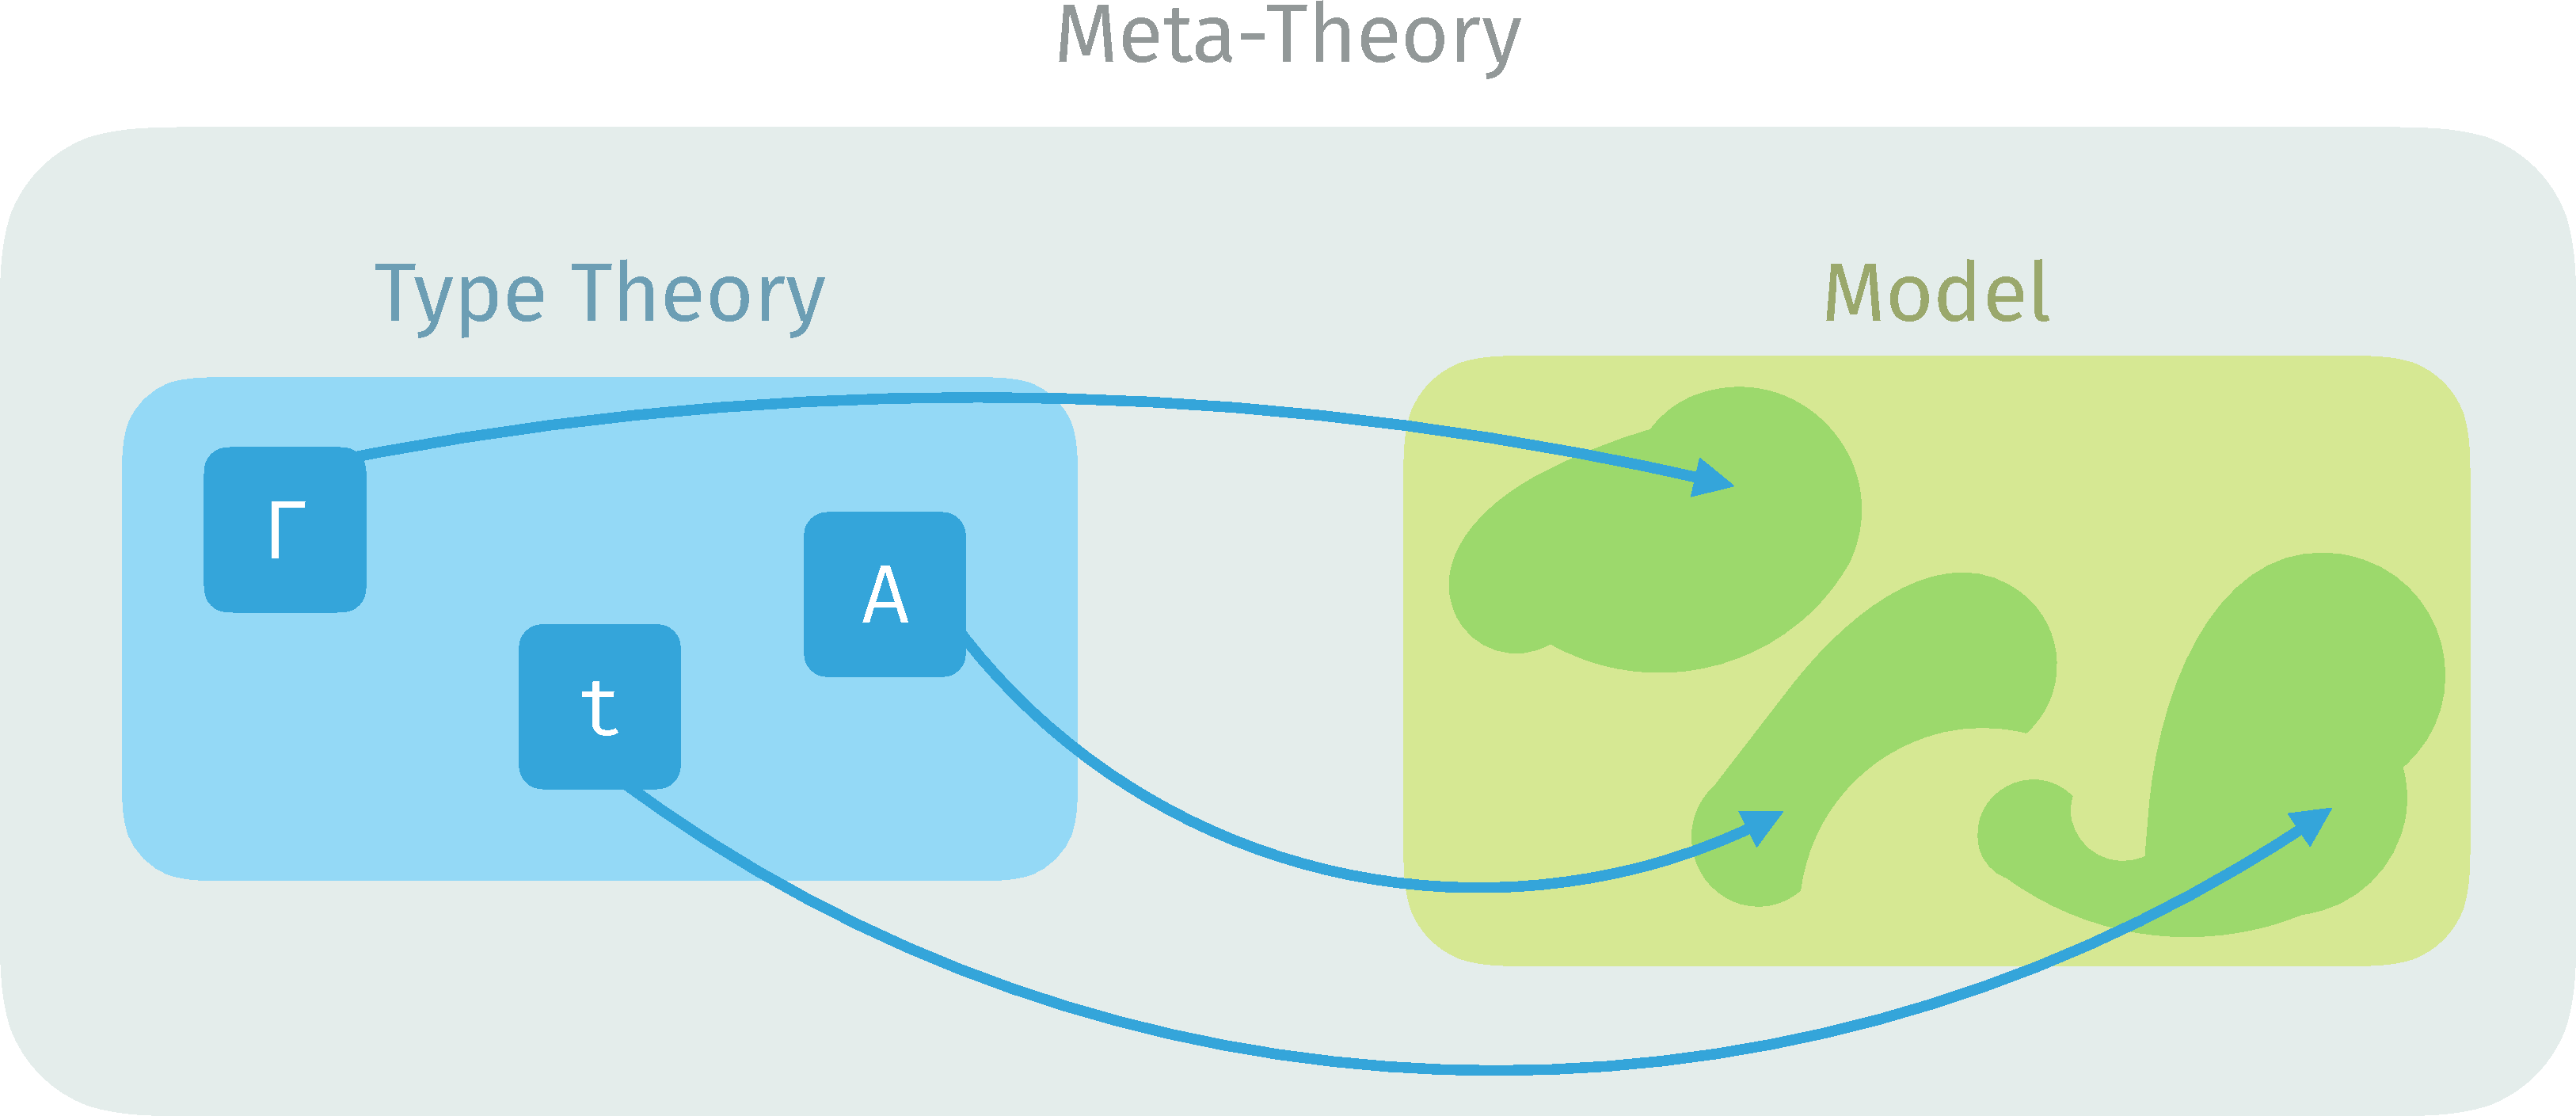
\includegraphics[width=0.9\textwidth]{model}
\end{figure}
To be more precise, a model is given by a class of objects to interpret
contexts, one for terms and one for types; but a model also provides an
interpretation to judgments in such a way that the interpretation is coherent.

\subsection{What can be proved using models}

\paragraph{Consistency.}

I already briefly mentioned this but the main point of models is to prove
consistency of a theory, relying on the already \emph{known} consistency of the
theory in which lives the model... At least in principle. It is however very
rare\sidenote{Impossible?} to \emph{know} that a theory is consistent, instead
we should see it as a theory we \emph{trust}, typically a theory that's widely
accepted as beeing consistent by the community of mathematicians.
This also applies to the meta-theory in which we show that the interpretation is
correct. As such it is best to keep it as simple as possible to avoid relying on
the consistency of too complicated objects.

\paragraph{Independence.}

Another interesing application of models is showing \emph{independence} of a
proposition.

\begin{definition}[Independent proposition]
  A proposition \(P\) is said to be independent from a theory \cT when neither
  \(P\) nor \(\neg P\) can be proven within \cT.
\end{definition}

A way to prove that some \(P\) is independent from \cT is to give a model of \cT
which validates \(P\) and another model which invalidates it (or validates
\(\neg P\)). Indeed if any one of \(P\) or \(\neg P\) %, let's say \(P\),
could be proven in \cT, then it would be valid in both models, leading to
at least one of them being inconsistent.

The fact that a proposition can neither be validated or invalidated in a theory
can come as surprising for some, especially in a classical mindset.
\reminder[-1.8cm]{Classical logic}{
  Classical logic is often characterised by the presence of the \acrshort{LEM}
  which consists in a proof of \(A \vee \neg A\).
}
Gödel's incompleteness theorems have to do with this.

\subsection{Gödel's incompleteness theorems}

\todo{Is it really the place? Should it even go in the proof theory chapter?}

\section{Set-theoretic models}

Set-theoretic models are models of type-theory where types are interpreted as
sets. For instance the type \(A \to B\) will be interpreted as the set of
set-theoretic functions from the interpretation of \(A\) to the interpretation
of \(B\):
\marginnote[0.2cm]{
  It is usual to write \(\transl{A}\) for the interpretation of \(A\).
}
\[
  \transl{A \to B} \coloneqq \setfun{\transl{A}}{\transl{B}})
\]
\todo{I'm missing a ref here on how to do this...}

\section{Categorical models}

Categorical models are one of the most used way of defining models for type
theories. There are several notions of categorical models:
contextual categories~\sidecite[-0.9cm]{cartmell1986generalised} from which stem
categories with attributes~\sidecite[0.2cm]{hofmann1994interpretation} and
C-systems~\sidecite[0.9cm]{voevodsky2016subsystems},
\acrfullpl{CwF}~\sidecite[1.7cm]{dybjer1995internal}, and more\dots
I will focus on \acrshortpl{CwF} in this document.

\subsection{Categories with families}

A \acrshort{CwF} is given by
\begin{enumerate}
  \item a collection of objects (or contexts) \(\Con\);
  \item morphisms (or substitutions) \(\sigma : \Ga \to \D\) between contexts
  \(\Ga, \D : \Con\);
  \item for each context \(\Ga : \Con\), a collection \(\CTy\ \Ga\) of types in
  that context;
  \item for each context \(\Ga : \Con\) and type \(A : \CTy\ \Ga\), a collection
  \(\CTm\ \Ga\ A\) of terms of type \(A\);
  \item an operation of substitution for types taking \(\sigma : \Ga \to \D\)
  and a type \(A : \CTy\ \D\) to type \(A[\sigma] : \CTy\ \Ga\);
  \item \label{item:term-subst} a similar substitution operation on terms taking
  \(\sigma : \Ga \to \D\) and a term \(t : \CTm\ \D\ A\) to term
  \(t[\sigma] : \CTm\ \Ga\ A[\sigma]\);
  \item a terminal object representing the empty context \(\ctxempty : \Con\);
  \item an extension operation taking \(\Ga : \Con\) and \(A : \CTy\ \Ga\)
  to a new object \(\Ga, A : \Con\) together with a morphism
  \(\pp : \Ga, A \to \Ga\) and a term \(\pq : \CTm\ (\Ga, A)\ A[\pp]\);
  \item an operation taking \(\sigma : \Ga \to \D\) and term
  \(a : \CTm\ \Ga\ A[\sigma]\) to substitution \(\sigma, a : \Ga \to \D, A\)
  such that \(\pp \circ (\sigma, a) = \sigma\) and \(\pq[\sigma, a] = a\).
\end{enumerate}
The two first have to give the structure of category, this in particular means
that there is an identity substitution, and associative composition of those.

The category \(\Set\) of sets is a \acrshort{CwF}:
\marginnote[3.8cm]{
  \ref{item:term-subst} holds because for every \(\gamma \in \Ga\),
  \[
    (t \circ \sigma)(\gamma) = t(\sigma(\gamma)) \in A_{\sigma(\gamma)}
    = A[\sigma]_\gamma
  \]
}
\begin{enumerate}
  \item objects are sets;
  \item substitutions are set-theoretic functions, composed as functions;
  \item types in \(\CTy\ \Ga\) are sets indexed by \(\Ga\);
  \item terms of \(\CTm\ \Ga\ A\) are choice functions
  \(t \in \setfun{\Ga}{\bigcup_{\gamma \in \Ga} A_\gamma}\) such that
  \(t(\gamma) \in A_\gamma\) for every \(\gamma \in \Ga\);
  \item given \(\sigma : \Ga \to \D\) and \(A : \CTy\ \D\), \(A[\sigma]\)
  is defined as the \(\Ga\)-index family \((A_{\sigma(\gamma)})_\gamma\);
  \item given \(\sigma : \Ga \to \D\) and \(t : \CTm\ \D\ A\), \(t[\sigma]\)
  is defined as the choice function \(t \circ \sigma\);
  \item the empty context is given as the singleton \(\{ \emptyset \}\);
  \item given \(\Ga : \Con\) and \(A : \CTy\ \Ga\), \(\Ga, A\) is defined as
  the disjoint union \(\amalg_{\gamma \in \Ga} A_\gamma\), \(\pp\) and \(\pq\)
  are defined as the first and second projection respectively;
  \item given \(\sigma : \Ga \to \D\) and \(a : \CTm\ \Ga\ A[\sigma]\),
  \(\sigma, a\) is defined as the function
  \(\gamma \mapsto (\sigma(\gamma), a)\) which verifies the conditions.
\end{enumerate}

Right now this only interprets a type theory with no type or term constructors

\subsection{Cardinal model}

\section{Type-theoretic models}

\todo{Cat models fall in this too}
\todo{translations, syntactical models, standard model}